\documentclass[12pt]{amsart}
\usepackage[left=0.5in, right=0.5in, bottom=0.75in, top=0.75in]{geometry}
\usepackage[english]{babel}
\usepackage[utf8x]{inputenc}
\usepackage{amsmath,amssymb,amsthm}
\usepackage{enumerate}
\usepackage{graphicx}
\usepackage{tikz}
\usepackage{pgfplots}
\pgfplotsset{compat = newest}
\usepgfplotslibrary{fillbetween}

\begin{document}
\raggedbottom

\noindent{\large OPER 610 - Linear Programming %
	% Lesson X %
	(Due Jan X at 10am)}
\hspace{\fill} {\large B. Hosley}
\bigskip


%%%%%%%%%%%%%%%%%%%%%%%
\setcounter{section}{5}
\setcounter{subsection}{34}
\subsection{}
Let \(\mathbf{A} = \begin{bmatrix} 1 & 1 \\ 0 & 2 \\ -1 & 4 \end{bmatrix}\)
and \(\mathbf{c} = (-1,5) \).
Which of the following two systems has a solution?
\begin{align*}
	System\ 1: \mathbf{Ax}\leq\mathbf{0},& \qquad \mathbf{cx}>0; \\
	System\ 2: \mathbf{wA}=\mathbf{c}& \qquad \mathbf{w}\geq\mathbf{0}.
\end{align*}

\bigskip
\textit{Solution:}

Evaluating system 1:
\begin{align*}
\intertext{From $\mathbf{Ax}\leq\mathbf{0}$ we get}
	x_1 + x_2 &\leq 0 \\
	  2x_2 & \leq 0 \\
	-x_1 + 4x_2 &\leq 0, \\
\intertext{and from $\mathbf{cx}>0$ we get}
	-x_1 + 5x_2 &> 0. \\
\intertext{Combining the third and fourth inequality we see}
	-x_1 + 4x_2 < -x_1 + 5x_2
\intertext{which simplifies to}
	x_2 > 0
\intertext{which is in direct contradiction to the second inequality above, namely,}
	2x_2 & \leq 0.
\end{align*}

Evaluating system 2:
\begin{align*}
\intertext{From $\mathbf{wA}=\mathbf{c}$ we get}
	w_1 \begin{bmatrix} 1 \\ 1\end{bmatrix} + 
	w_2 \begin{bmatrix} 0 \\ 2\end{bmatrix} + 
	w_3 \begin{bmatrix} -1 \\ 4\end{bmatrix} &= 
	\begin{bmatrix} -1 \\ 5\end{bmatrix}.
\end{align*}
By inspection, one feasible solution is
\(w_1 = 0, \ w_2 = 1/2, \text{ and, } w_3 = 1\).

\begin{center}
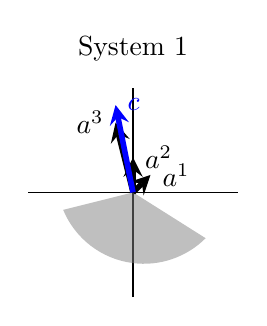
\begin{tikzpicture}
	\begin{axis}[
		title=System 1,
		xmin = -6, xmax = 6, xtick distance = 10,
		ymin = -6, ymax = 6, ytick distance = 10,
		grid = both,
		axis lines = center,
		ticks = none,
		major grid style = {},
		width = 0.35\textwidth,
		height = 0.35\textwidth,
		axis line style={-}
		]
		\draw[transparent, fill=gray, fill opacity=0.5] (0,0) -- (-4,-1) arc (202.5:315:5) --cycle;
		\addplot [
		black, line width=2pt,
		quiver={u=\thisrow{u},v=\thisrow{v}},
		stealth-,
		nodes near coords,
		point meta=explicit symbolic,
		coordinate style/.from= \thisrow{style},
		] table [meta=label] {
			x y u v label	style
			1 1 -1 -1 $a^1$	right
			0 2 0 -2 $a^2$	right
		   -1 4 1 -4 $a^3$	left
		};
		\addplot [
		blue, line width=2pt,
		quiver={u=\thisrow{u},v=\thisrow{v}},
		stealth-,
		nodes near coords,
		point meta=explicit symbolic,
		coordinate style/.from= \thisrow{style},
		] table [meta=label] {
			x y u v label	style
			-1 5 1 -5 $c$	right
		};
	\end{axis}
\end{tikzpicture} \hspace{5em}
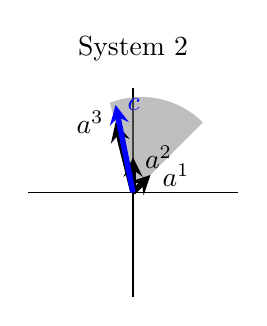
\begin{tikzpicture}
	\begin{axis}[
		title=System 2,
		xmin = -6, xmax = 6, xtick distance = 10,
		ymin = -6, ymax = 6, ytick distance = 10,
		grid = both,
		axis lines = center,
		ticks = none,
		major grid style = {},
		width = 0.35\textwidth,
		height = 0.35\textwidth,
		axis line style={-}
		]
		\draw[transparent, fill=gray, fill opacity=0.5] (0,0) -- (4,4) arc (45:111:5) --cycle;
		\addplot [
		black, line width=2pt,
		quiver={u=\thisrow{u},v=\thisrow{v}},
		stealth-,
		nodes near coords,
		point meta=explicit symbolic,
		coordinate style/.from= \thisrow{style},
		] table [meta=label] {
			x y u v label	style
			1 1 -1 -1 $a^1$	right
			0 2 0 -2 $a^2$	right
			-1 4 1 -4 $a^3$	left
		};
		\addplot [
		blue, line width=2pt,
		quiver={u=\thisrow{u},v=\thisrow{v}},
		stealth-,
		nodes near coords,
		point meta=explicit symbolic,
		coordinate style/.from= \thisrow{style},
		] table [meta=label] {
			x y u v label	style
			-1 5 1 -5 $c$	right
		};
	\end{axis}
\end{tikzpicture}
\end{center}

\clearpage
\setcounter{subsection}{40}
\subsection{}
Write the KKT optimality conditions for each of the following problems:
\begin{enumerate}
	\item[a.] \begin{align*}
		\text{Maximize }\,\,\ \mathbf{cx} & \hspace{75ex}\\
		\text{subject to  } \mathbf{Ax} &\leq \mathbf{b} \\
		\mathbf{x} &\geq \mathbf{0}.
	\end{align*} \vspace{-5ex}
	\item[c.] \begin{align*}
		\text{Minimize }\,\,\ \mathbf{cx} & \hspace{75ex}\\
		\text{subject to  } \mathbf{Ax} &\leq \mathbf{b} \\
		\mathbf{x} &\geq \mathbf{0}.
	\end{align*} \vspace{-5ex}
	\item[d.]\begin{align*}
		\text{Minimize }\quad \mathbf{cx} & \hspace{75ex}\\
		\text{subject to  } \mathbf{A_1x} &= \mathbf{b_1} \\
		\mathbf{A_2x} &\geq \mathbf{b_2} \\
		\mathbf{x} &\geq \mathbf{0}.
	\end{align*} \vspace{-5ex}
	\item[e.] \begin{align*}
		\text{Minimize }\,\ \mathbf{cx} & \hspace{75ex}\\
		\text{subject to  } \mathbf{Ax} &= \mathbf{b} \\
		\mathbf{x} &\leq \mathbf{u} \\
		\mathbf{x} &\geq \boldsymbol{\ell}.
	\end{align*} \vspace{-5ex}
\end{enumerate}

\bigskip
\textit{Solution:}

\begin{enumerate}
	\item[a.]
	\underline{Primal:}
	\begin{align*}
		\mathbf{Ax} &\leq \mathbf{b} \hspace{25ex}\\
		\mathbf{x} &\geq \mathbf{0}.
	\end{align*}
	\underline{Dual:}
	\begin{align*}
		\mathbf{wA} - \mathbf{v} &= \mathbf{c} \hspace{25ex}\\
		\mathbf{w} &\geq \mathbf{0} \\
		\mathbf{v} &\geq \mathbf{0}.
	\end{align*}
	\underline{Complementary Slackness:}
	\begin{align*}
		\mathbf{w}(\mathbf{b}-\mathbf{Ax}) &=0,
	\intertext{and}
		(\mathbf{wA}-\mathbf{c})\mathbf{x} &=0,
	\intertext{and}
		\mathbf{vx} = 0.
	\end{align*}
	
	\item[c.]
	\underline{Primal:}
	\begin{align*}
		\mathbf{Ax} &\leq \mathbf{b} \hspace{25ex}\\
		\mathbf{x} &\geq \mathbf{0}.
	\end{align*}
	\underline{Dual:}
	\begin{align*}
		\mathbf{wA} + \mathbf{v} &= \mathbf{c} \hspace{25ex}\\
		\mathbf{w} &\leq \mathbf{0} \\
		\mathbf{v} &\leq \mathbf{0}.
	\end{align*}
	\underline{Complementary Slackness:}
	\begin{align*}
		\mathbf{w}(\mathbf{b}-\mathbf{Ax}) &=0,
		\intertext{and}
		(\mathbf{wA}-\mathbf{c})\mathbf{x} &=0,
		\intertext{and}
		\mathbf{vx} = 0.
	\end{align*}
	
	\item[d.]
	\underline{Primal:}
	\begin{align*}
		\mathbf{A_1x} &= \mathbf{b_1} \hspace{25ex}\\
		\mathbf{A_2x} &\geq \mathbf{b_2} \\
		\mathbf{x} &\geq \mathbf{0}.
	\end{align*}
	\underline{Dual:}
	\begin{align*}
		\mathbf{w}_1\mathbf{A}_1 + \mathbf{w}_2\mathbf{A}_2 - \mathbf{v} &= \mathbf{c} \hspace{25ex} \\
		\mathbf{w}_1 &\text{: unrestricted} \\
		\mathbf{w}_2 &\geq \mathbf{0} \\
		\mathbf{v} &\geq \mathbf{0}.
	\end{align*}
	\underline{Complementary Slackness:}
	\begin{align*}
		\mathbf{w}_2(\mathbf{A}_2\mathbf{x} - \mathbf{b}_2)  = \mathbf{0} \\
		\mathbf{vx} = 0
	\end{align*}
	
	\item[e.]
	\underline{Primal:}
	\begin{align*}
		\mathbf{Ax} &= \mathbf{b} \hspace{35ex}\\
		\mathbf{x} &\leq \mathbf{u} \\
		\mathbf{x} &\geq \boldsymbol{\ell}.
	\end{align*}
	\underline{Dual:}
	\begin{align*}
		\mathbf{wA}- \mathbf{u} + \mathbf{v} &= \mathbf{c} \hspace{35ex}\\
		\mathbf{wA}- \boldsymbol{\ell} - \mathbf{v} &= \mathbf{c} \\
		\mathbf{w} &:\text{ unrestricted}.
	\end{align*}
	\underline{Complementary Slackness:}
	\begin{align*}
		\mathbf{w}(\mathbf{Ax}-\mathbf{b}) &=0 \hspace{35ex}\\
		\mathbf{vx} &= 0
	\end{align*}
	
\end{enumerate}


\end{document}